\chapter{IDEX Instrument Description}
\label{chap:chap3}
\section{Overview}
The Interstellar Dust Experiment (IDEX) is a high-resolution impact ionization time-of-flight (TOF) mass spectrometer that provides the elemental composition and mass distributions of ISD and IDP particles. IDEX links the interstellar gas phase composition, as obtained with IMAP-Lo and through PUIs with CoDICE and SWAPI, with the makeup of ISD and IDP particles. 
\begin{figure}[H]
    \centering
    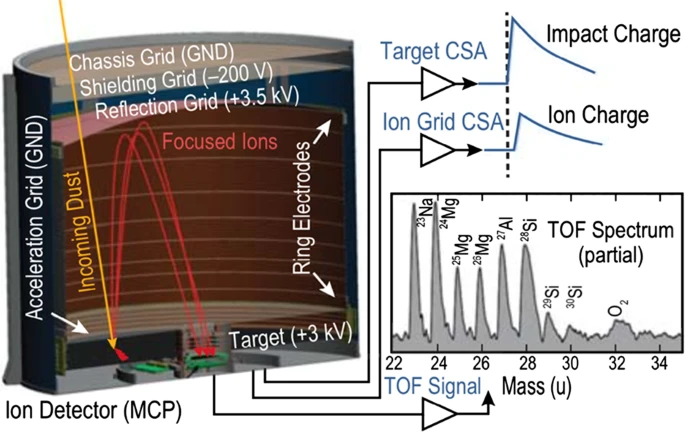
\includegraphics[width=\linewidth]{images/overview.png}
    \caption{An outline of the IDEX instrument and principle of operation. The three types of signals produced (ion grid, target and time-of-flight) are labeled and depicted by their corresponding hardware.}
    \label{fig:overview}
\end{figure}

IDEX is based on the heritage of past flight and laboratory instruments. Its operation principle is based on the impact ionization process.

IDEX has two components, an electronics enclosure and a sensor head with a large effective target area ($600$ cm$^2)$. The IDEX mechanical design consists of a simple Al shell structure that provides support for the biased electrodes of the TOF ion mass analyzer and the grids over its aperture. The centrally-located ion detector and the front-end charge sensitive amplifier are integrated into the bottom of the instrument.

 Individual dust particles entering the instrument pass through a set of grid electrodes and impact the target (Figure \ref{fig:overview}). The target is biased at +3 kV to provide positive ion acceleration and the reflectron-type ion optics are used to generate TOF compositional mass spectra. The impact-generated negative charges are collected on the target. An electrostatic field, shaped by a set of biased rings and a curved grid electrode, provides spatial and temporal focusing of the accelerated ions onto the central detector.


Target cleanliness is of high importance to be maintained throughout the fabrication, integration and operation of IDEX. The primary concern is the condensation of volatiles on the target. The mitigate this risk, 
IDEX has a one-time deployable door and its in-flight operation allows for the regular (once per months) use of heaters to raise the target temperature to 120 C over 8 hours in order to release any possible condensible contaminants. 

 
\section{Sensor Head}
An overview of the sensor head is shown in Figure \ref{fig:sensor}.

\begin{figure}[H]
    \centering
    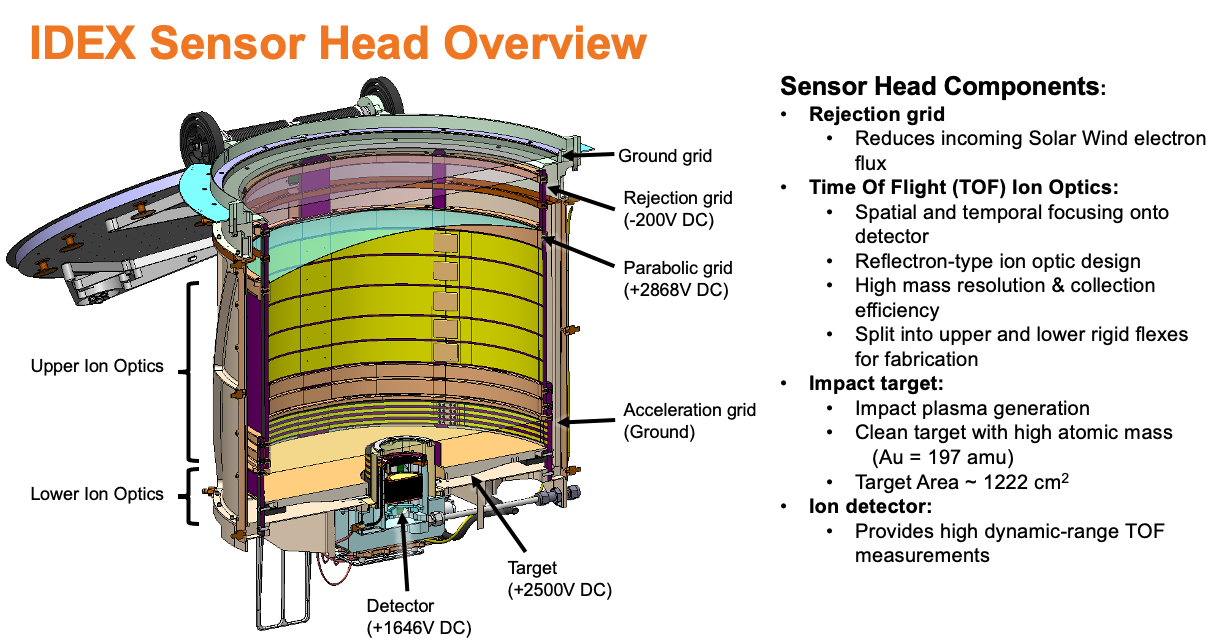
\includegraphics[width=\linewidth]{images/SensorHead.png}
    \caption{An outline of the IDEX instrument sensor head.}
    \label{fig:sensor}
\end{figure}

\section{Electronics}

The IDEX electronics leverage SUDA flight designs. The Decon/Actuator Board (DAB) is a new design that was added to control the door and decontamination heater.  The amplifier boards (CSA, Detector Buffer) were re-designed from the SUDA heritage instrument to meet the IDEX requirements for charge detection ranges. An overview of the IDEX electronics is depicted in Figure \ref{fig:elec}. 

\begin{figure}[H]
    \centering
    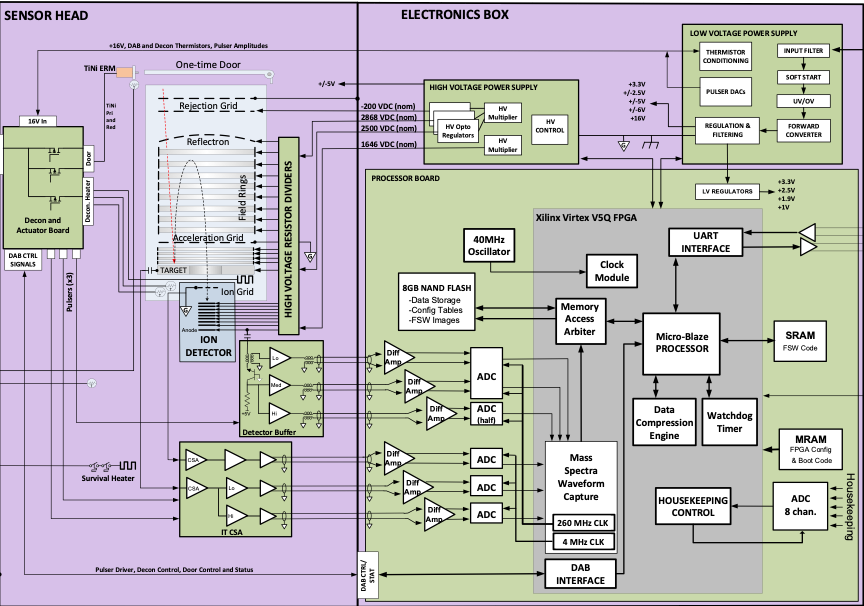
\includegraphics[width=\linewidth]{images/BlockDiagram.png}
    \caption{An outline of the IDEX instrument electronics system.}
    \label{fig:elec}
\end{figure}

%The electronics components relevant to the science data processing pipeline are the sensor head (excluding the Decon Actuator Board (DAB)) and the processor board. 

The 3 Time-of-Flight (TOF) gain stages, 2 Target CSA and 1 Ion grid CSA waveforms are the signals which the science data products are derived from. These constitute the packetized data accumulated in an 8 GB NAND flash and form the IDEX level 0 data product. 